\documentclass{article}
\usepackage{graphicx, amsfonts, amssymb, amsmath, amsthm, float} % Required for inserting images
\usepackage[english]{babel}
\usepackage[letterpaper,top=2cm,bottom=2cm,left=3cm,right=3cm,marginparwidth=1.75cm]{geometry}

\title{EE132 Lab 2}
\author{Andre Winkel, Russell Yang}
\date{\today}

\begin{document}
\maketitle

\begin{abstract}
    In this lab, we will use an encoder to measure speed. We will also implement low-pass filters in order to depict more accurate readings of the servo speed. We will use the principles of transfer functions in order to establish our cut-off frequencies, while maintaining an accurate representation of the servo speed.
\end{abstract}

\section{System built}
\begin{figure} [H]
    \centering
    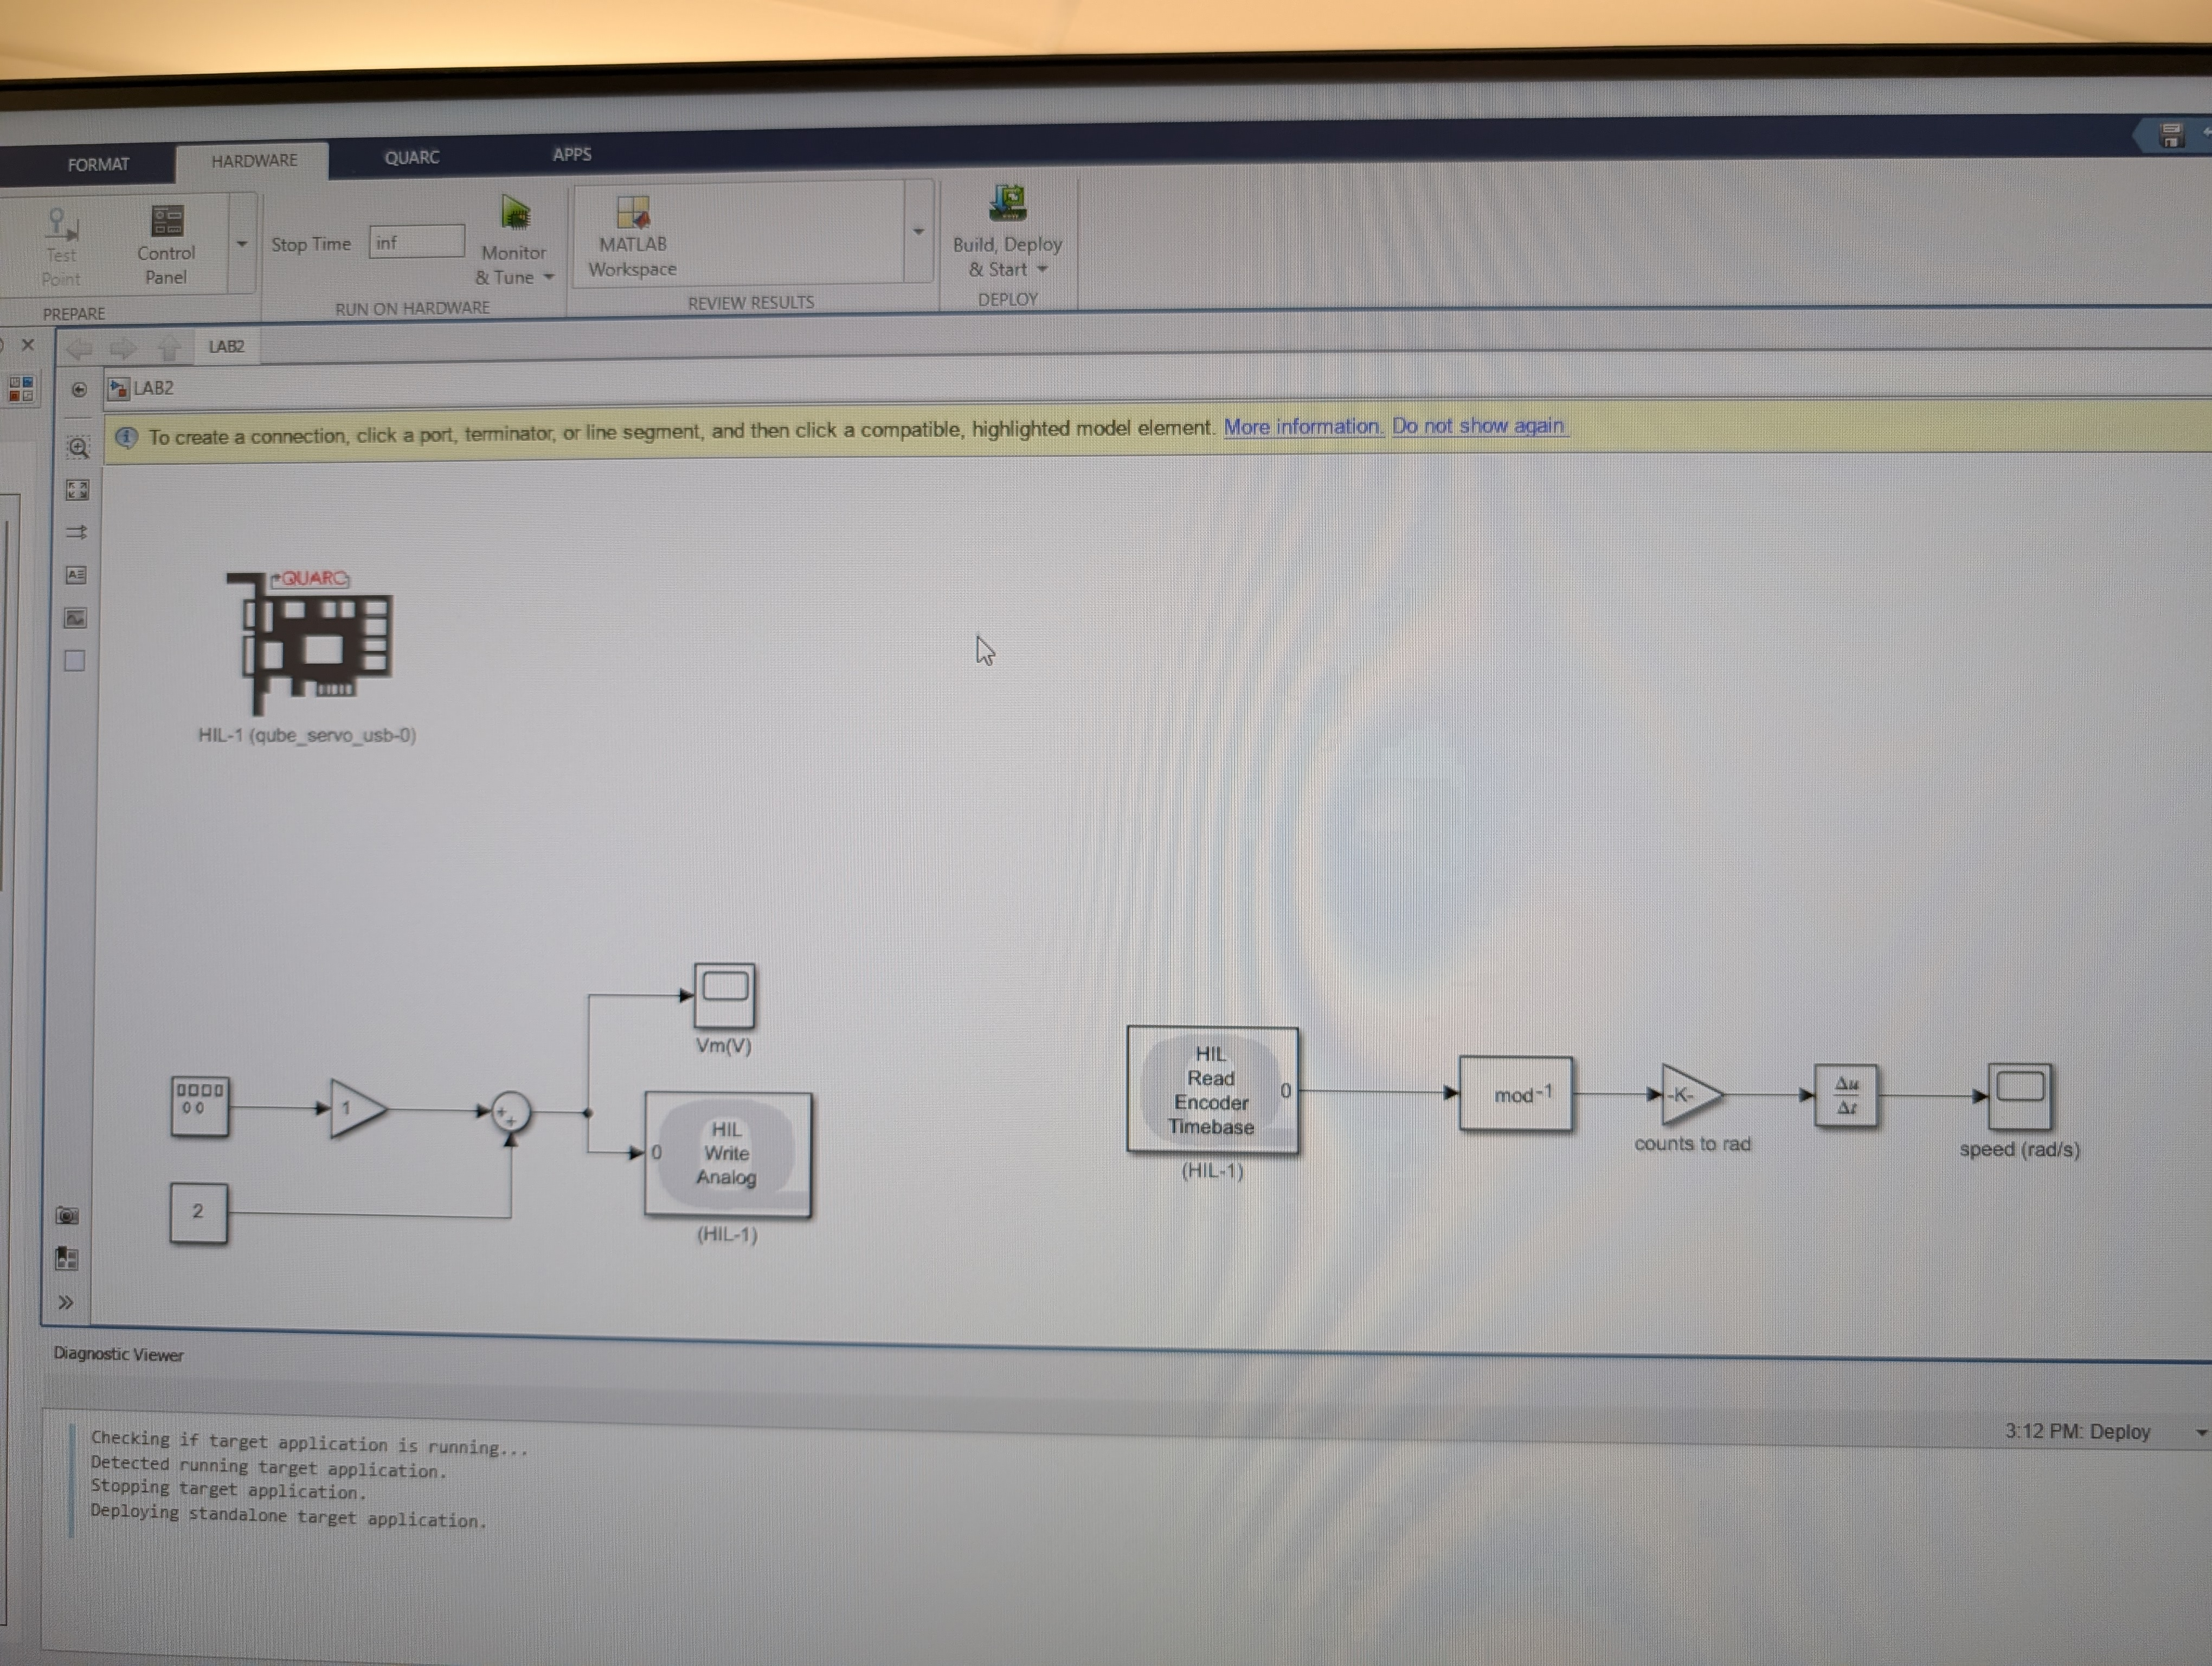
\includegraphics[width=0.5\linewidth]{1.jpg}
    \caption{The system excluding transfer function}
    \label{fig:1}
\end{figure}
Note here that our final system included a transfer function between the derivative and speed probe.

\section{In-Lab exercises and Results}
\subsection{Encoder gain}
In order to change the encoder calibration gain to measure the gear position in radians (instead of degrees), we must recall that a full rotation of the encoder results in a value of $2048$. Considering this and how we previously used a constant of $\frac{360}{2048}$ as a factor in order to obtain a measurement in degrees, we can assume that a conversion to radians will be as follows:
\begin{equation}
    (\frac{360}{2048})(\frac{\pi}{180}).
\end{equation}
Reducing,
\begin{equation}
    (\frac{360}{2048})(\frac{\pi}{180})=\frac{360\pi}{2048*180}=\frac{2\pi}{2048}=\frac{\pi}{1024}.
\end{equation}
We can verify this by multiplying it with the original value of a full rotation of the encoder, where we observe
\begin{equation}
    (\frac{\pi}{1024})(2048)=2\pi,
\end{equation}
which is a full rotation in radians.

\subsection{Encoder speed measurement} 

\begin{figure}[H]
    \centering
    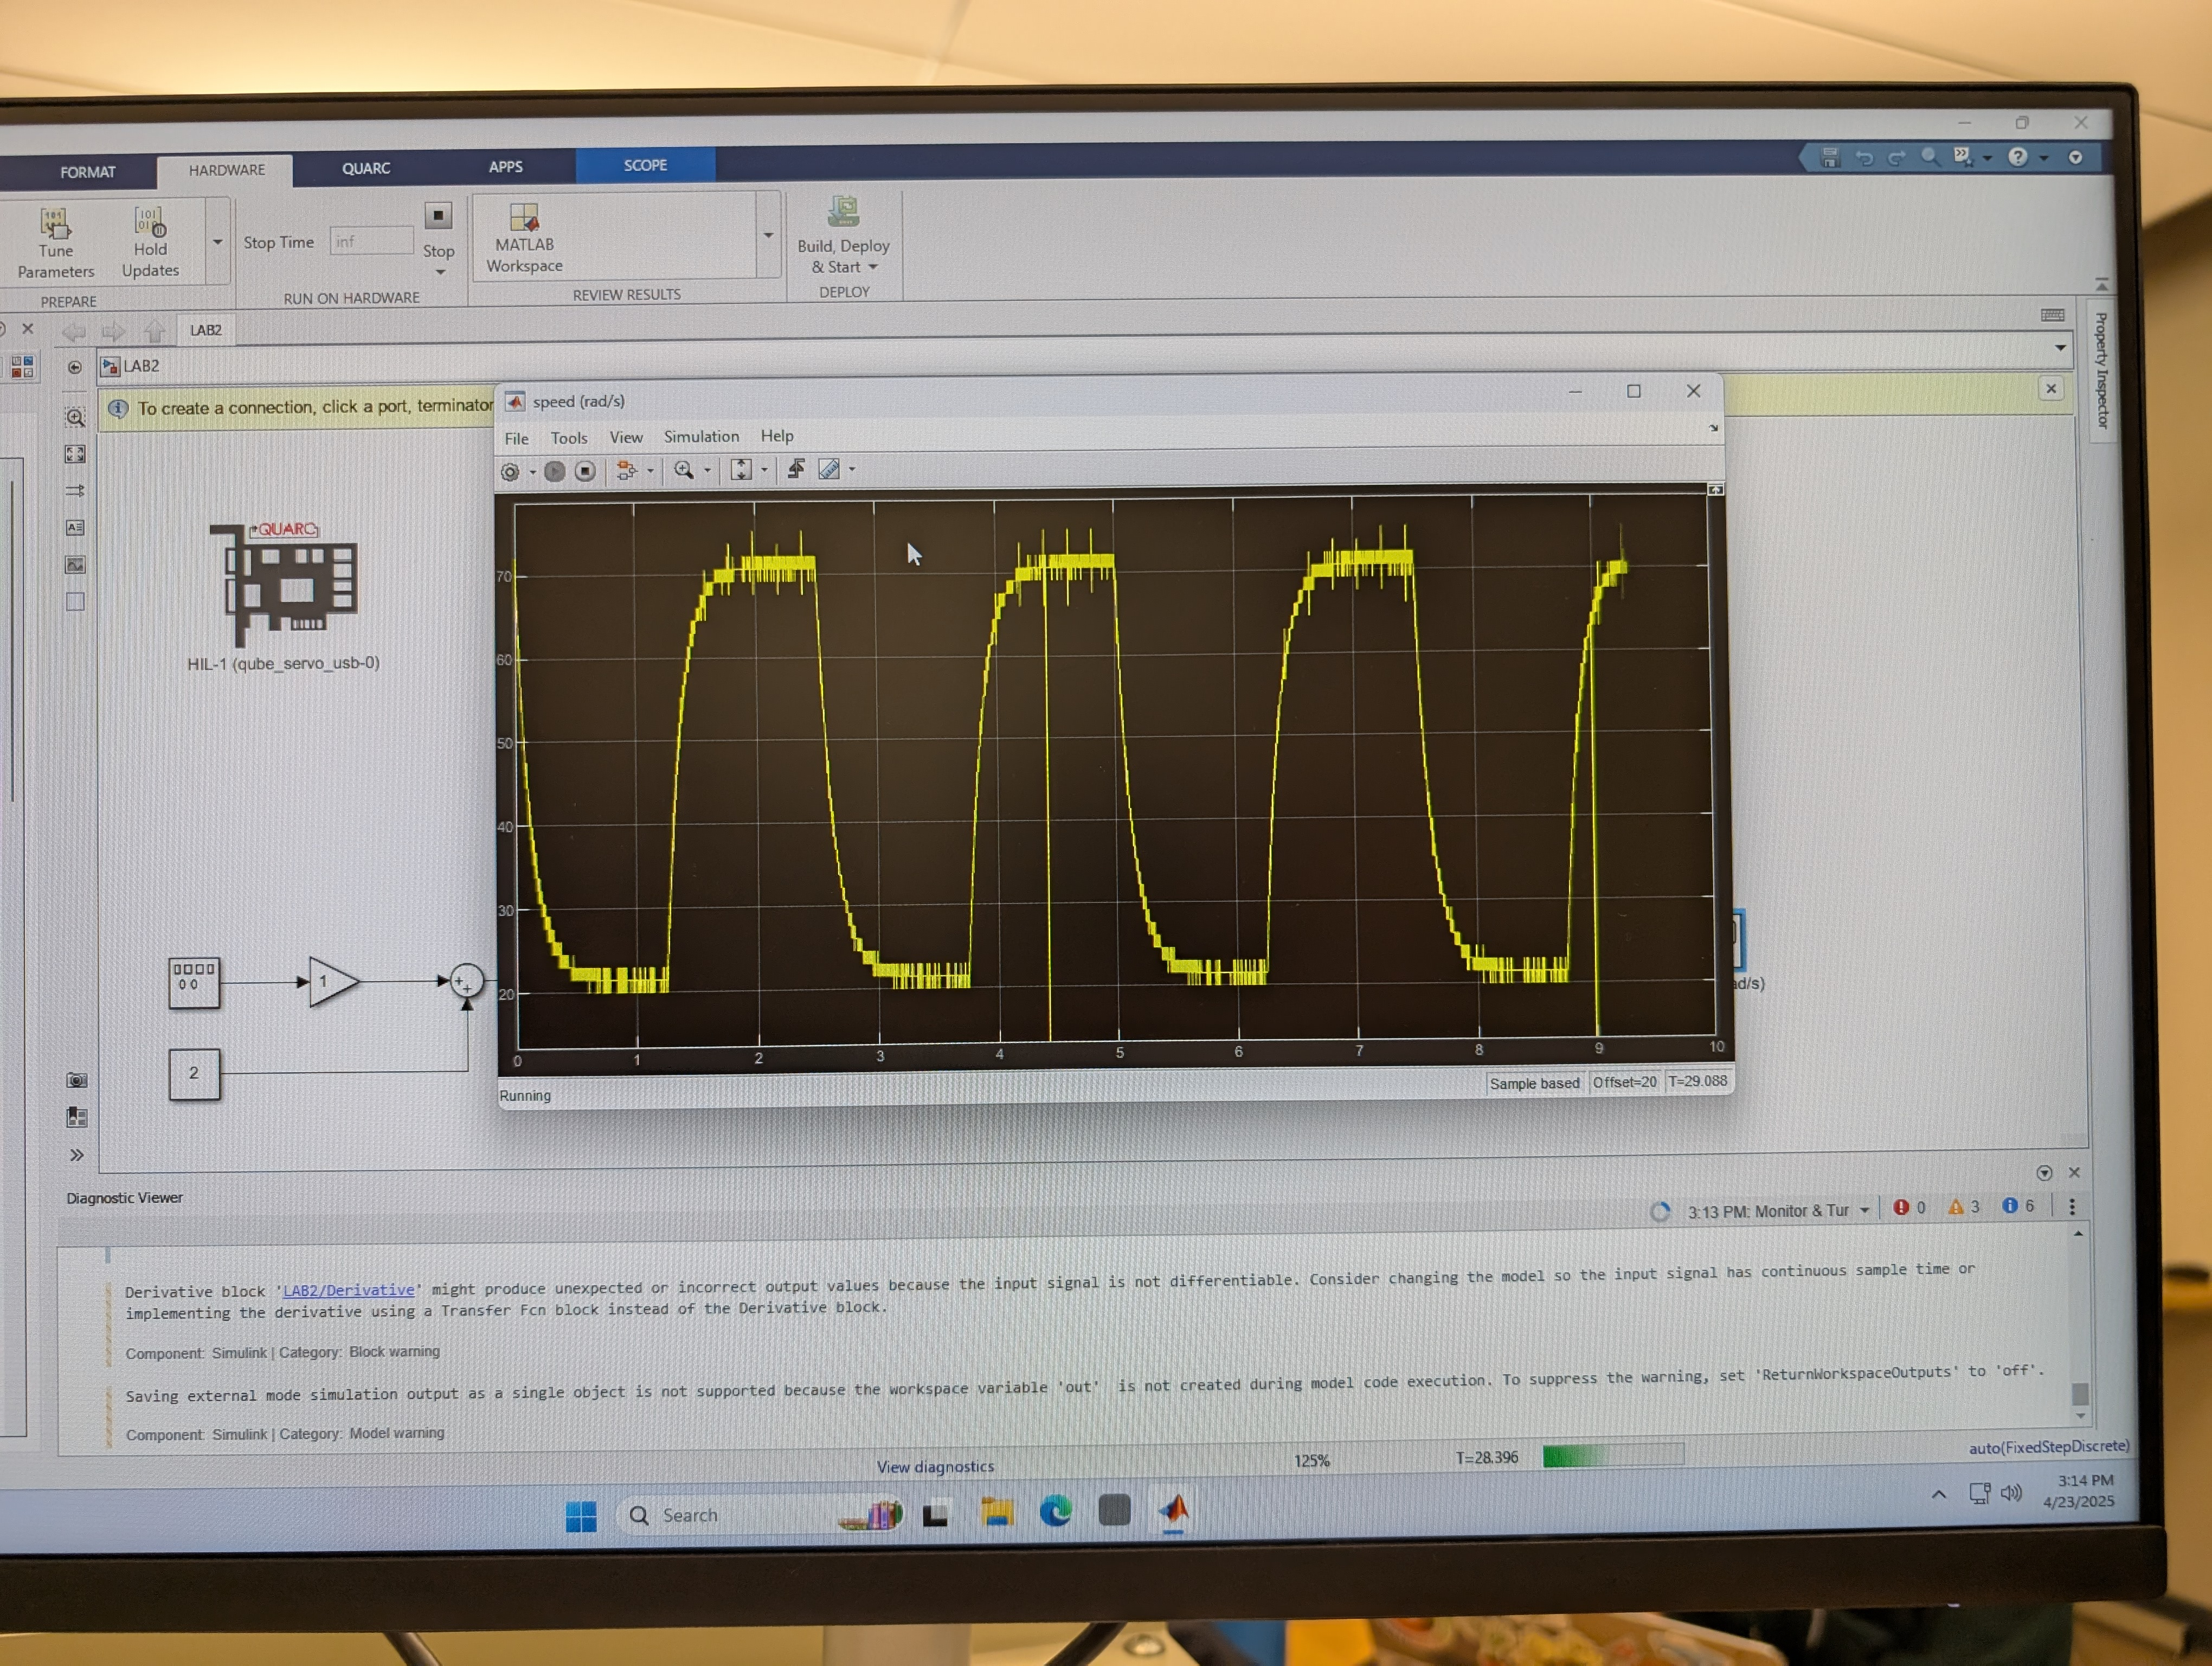
\includegraphics[width=0.49\linewidth]{2.jpg}
    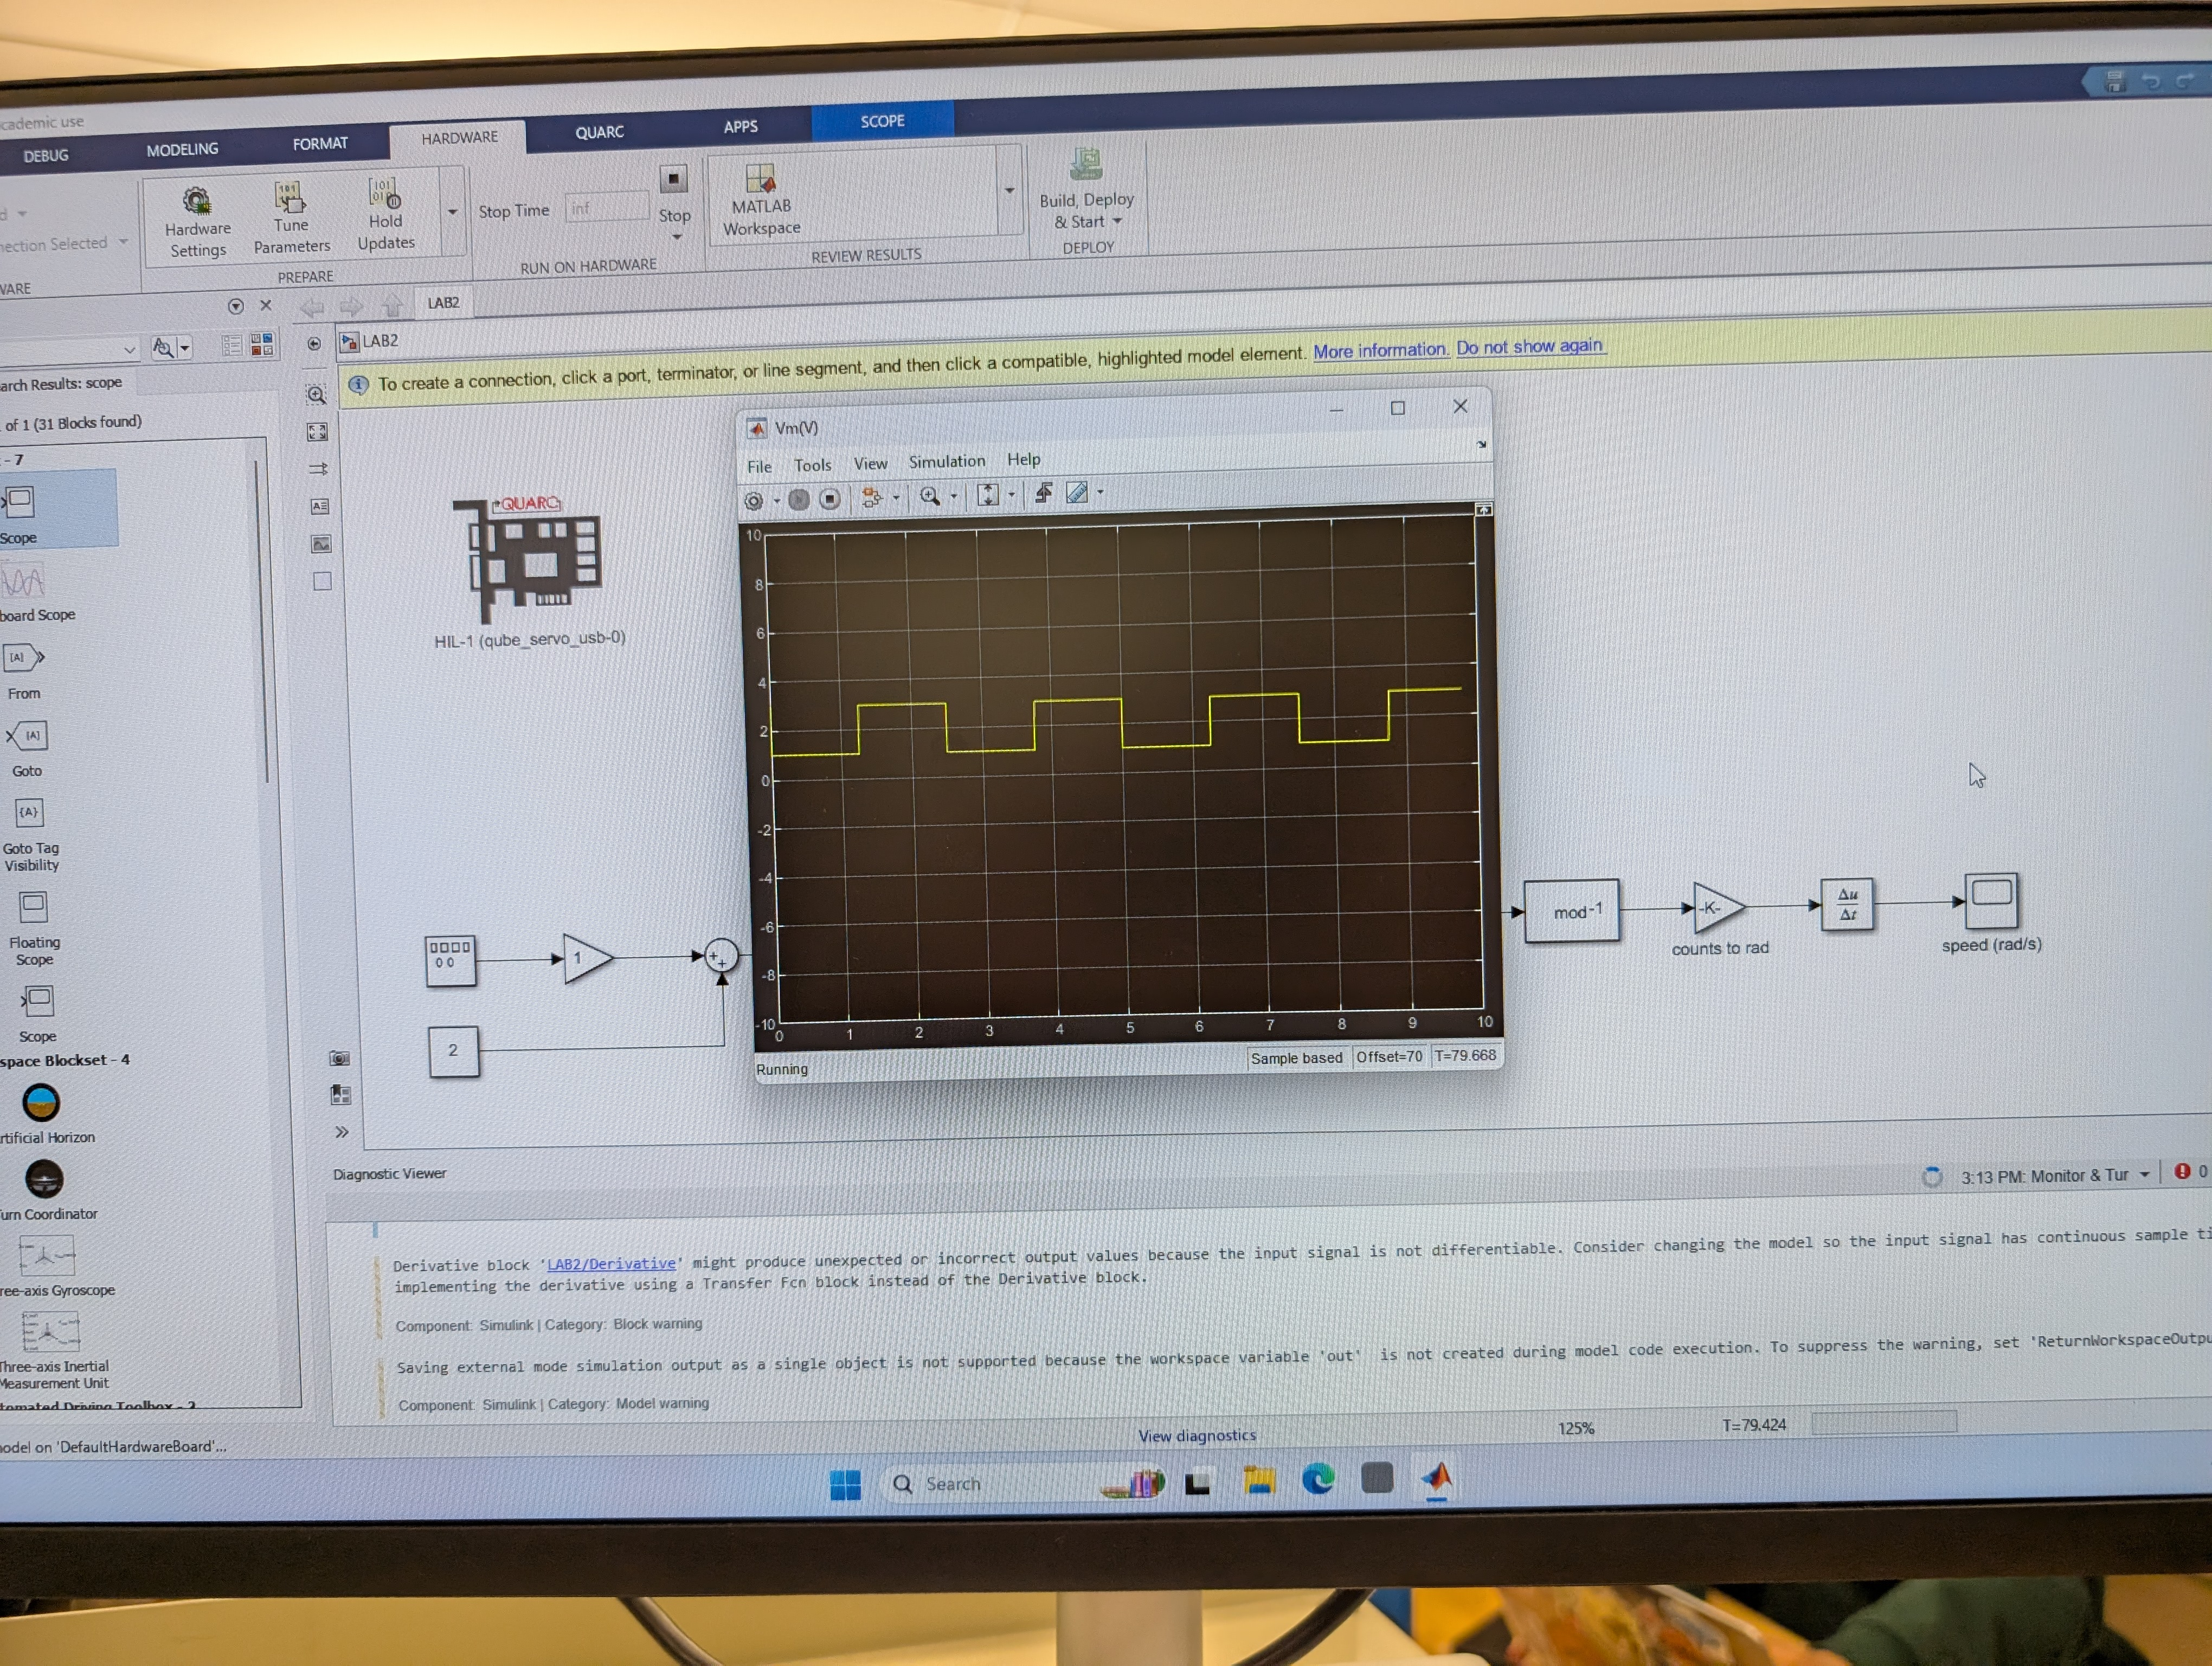
\includegraphics[width=0.49\linewidth]{3.jpg}
    \centering
    \caption{Encoder speed sample response}
    \label{fig:2}
\end{figure}

\subsection{Noise in encoder-based measurement}
We observe noise in our encoder speed measurement through the Simulink scope. The primary reason for such noise is that we are measuring the speed through taking the derivative of the encoder position with respect to time; Our method for deriving the speed from the position introduces noise, both in its nature but also because the position measurements are not fully, completely precise. Small artifacts in the position reading easily result in large artifacts in the speed. An additional reason for the larger noise is the occasional reset in the encoder position measurement, which causes a discontinuation.

\subsection{Filtering out high-frequency components from output}
A primary method we can use in order to reduce such noise is by implementing a low-pass filter after the derivative output, before the scope. Connecting it to both modules on their respective sides, we can set our \textit{Transfer Fcn} block to $\frac{50}{s+50}$.

\subsection{Analyzing the filtered response}
After implementing the low pass filter, we can observe the following plot of the velocity and the reference voltage:
\begin{figure}[H]
    \centering
    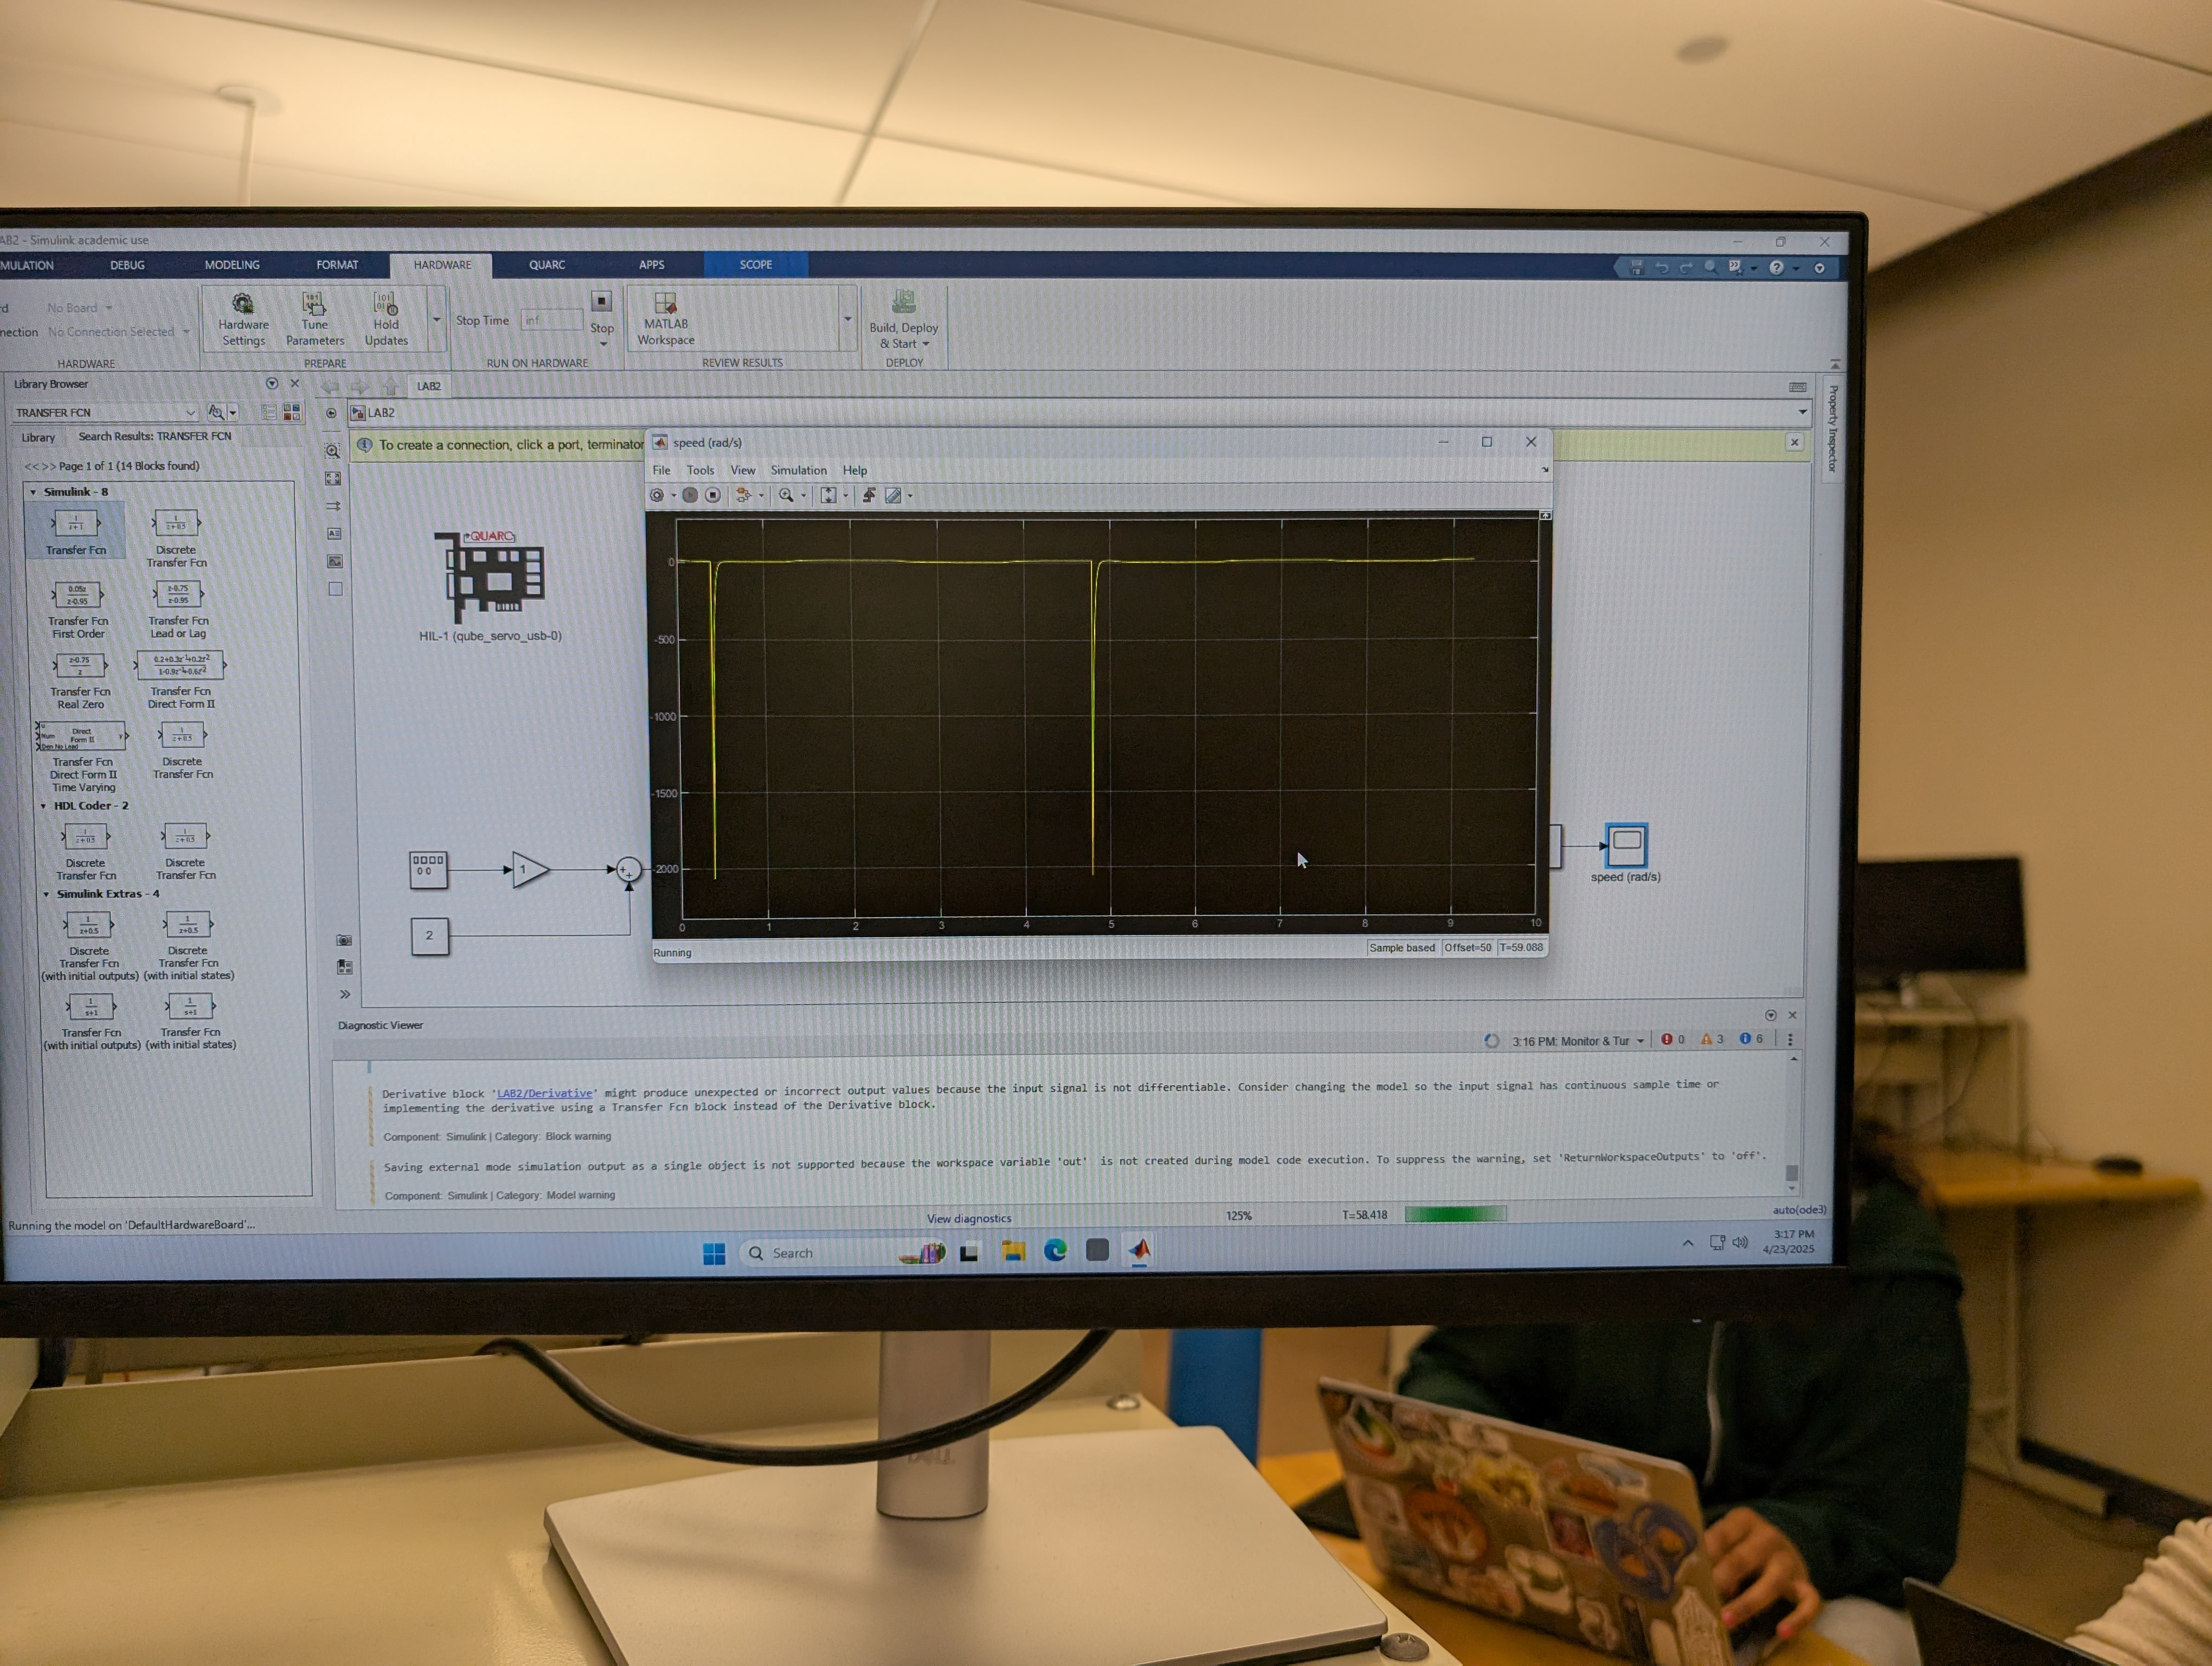
\includegraphics[width=0.49\linewidth]{5.jpg}
    \includegraphics[width=0.49\linewidth]{4.jpg}

    \centering
    \caption{Filtered response with $\omega_f=50$}
    \label{fig:3}
\end{figure}
We can therefore conclude that the measurement has improved. When fully zoomed into the filtered speed graph, we can see a more stable measurement. Though we still observe the original extremities that were present in the original, our important values are much cleaner and the high-frequency noise is filtered out.

\subsection{Cutoff frequency of low pass}
Using our transfer function,
\begin{equation}
    F(s)=\frac{50}{s+50},
\end{equation}
we can directly extract $\omega_f=50$, which is the cutoff frequency of the filter in $\frac{\text{rad}}{\text{s}}$. To convert to $\text{Hz}$, we can say 
\begin{equation}
    f_c=\frac{\omega_f}{2\pi}=\frac{25}{\pi} \approx 7.958\text{Hz}
\end{equation}
\subsection{Varying the cutoff frequency}
Below, the speed plots with $\omega_f=10$ and $\omega_f=200$ are displayed. 
\begin{figure}[H]
    \centering
    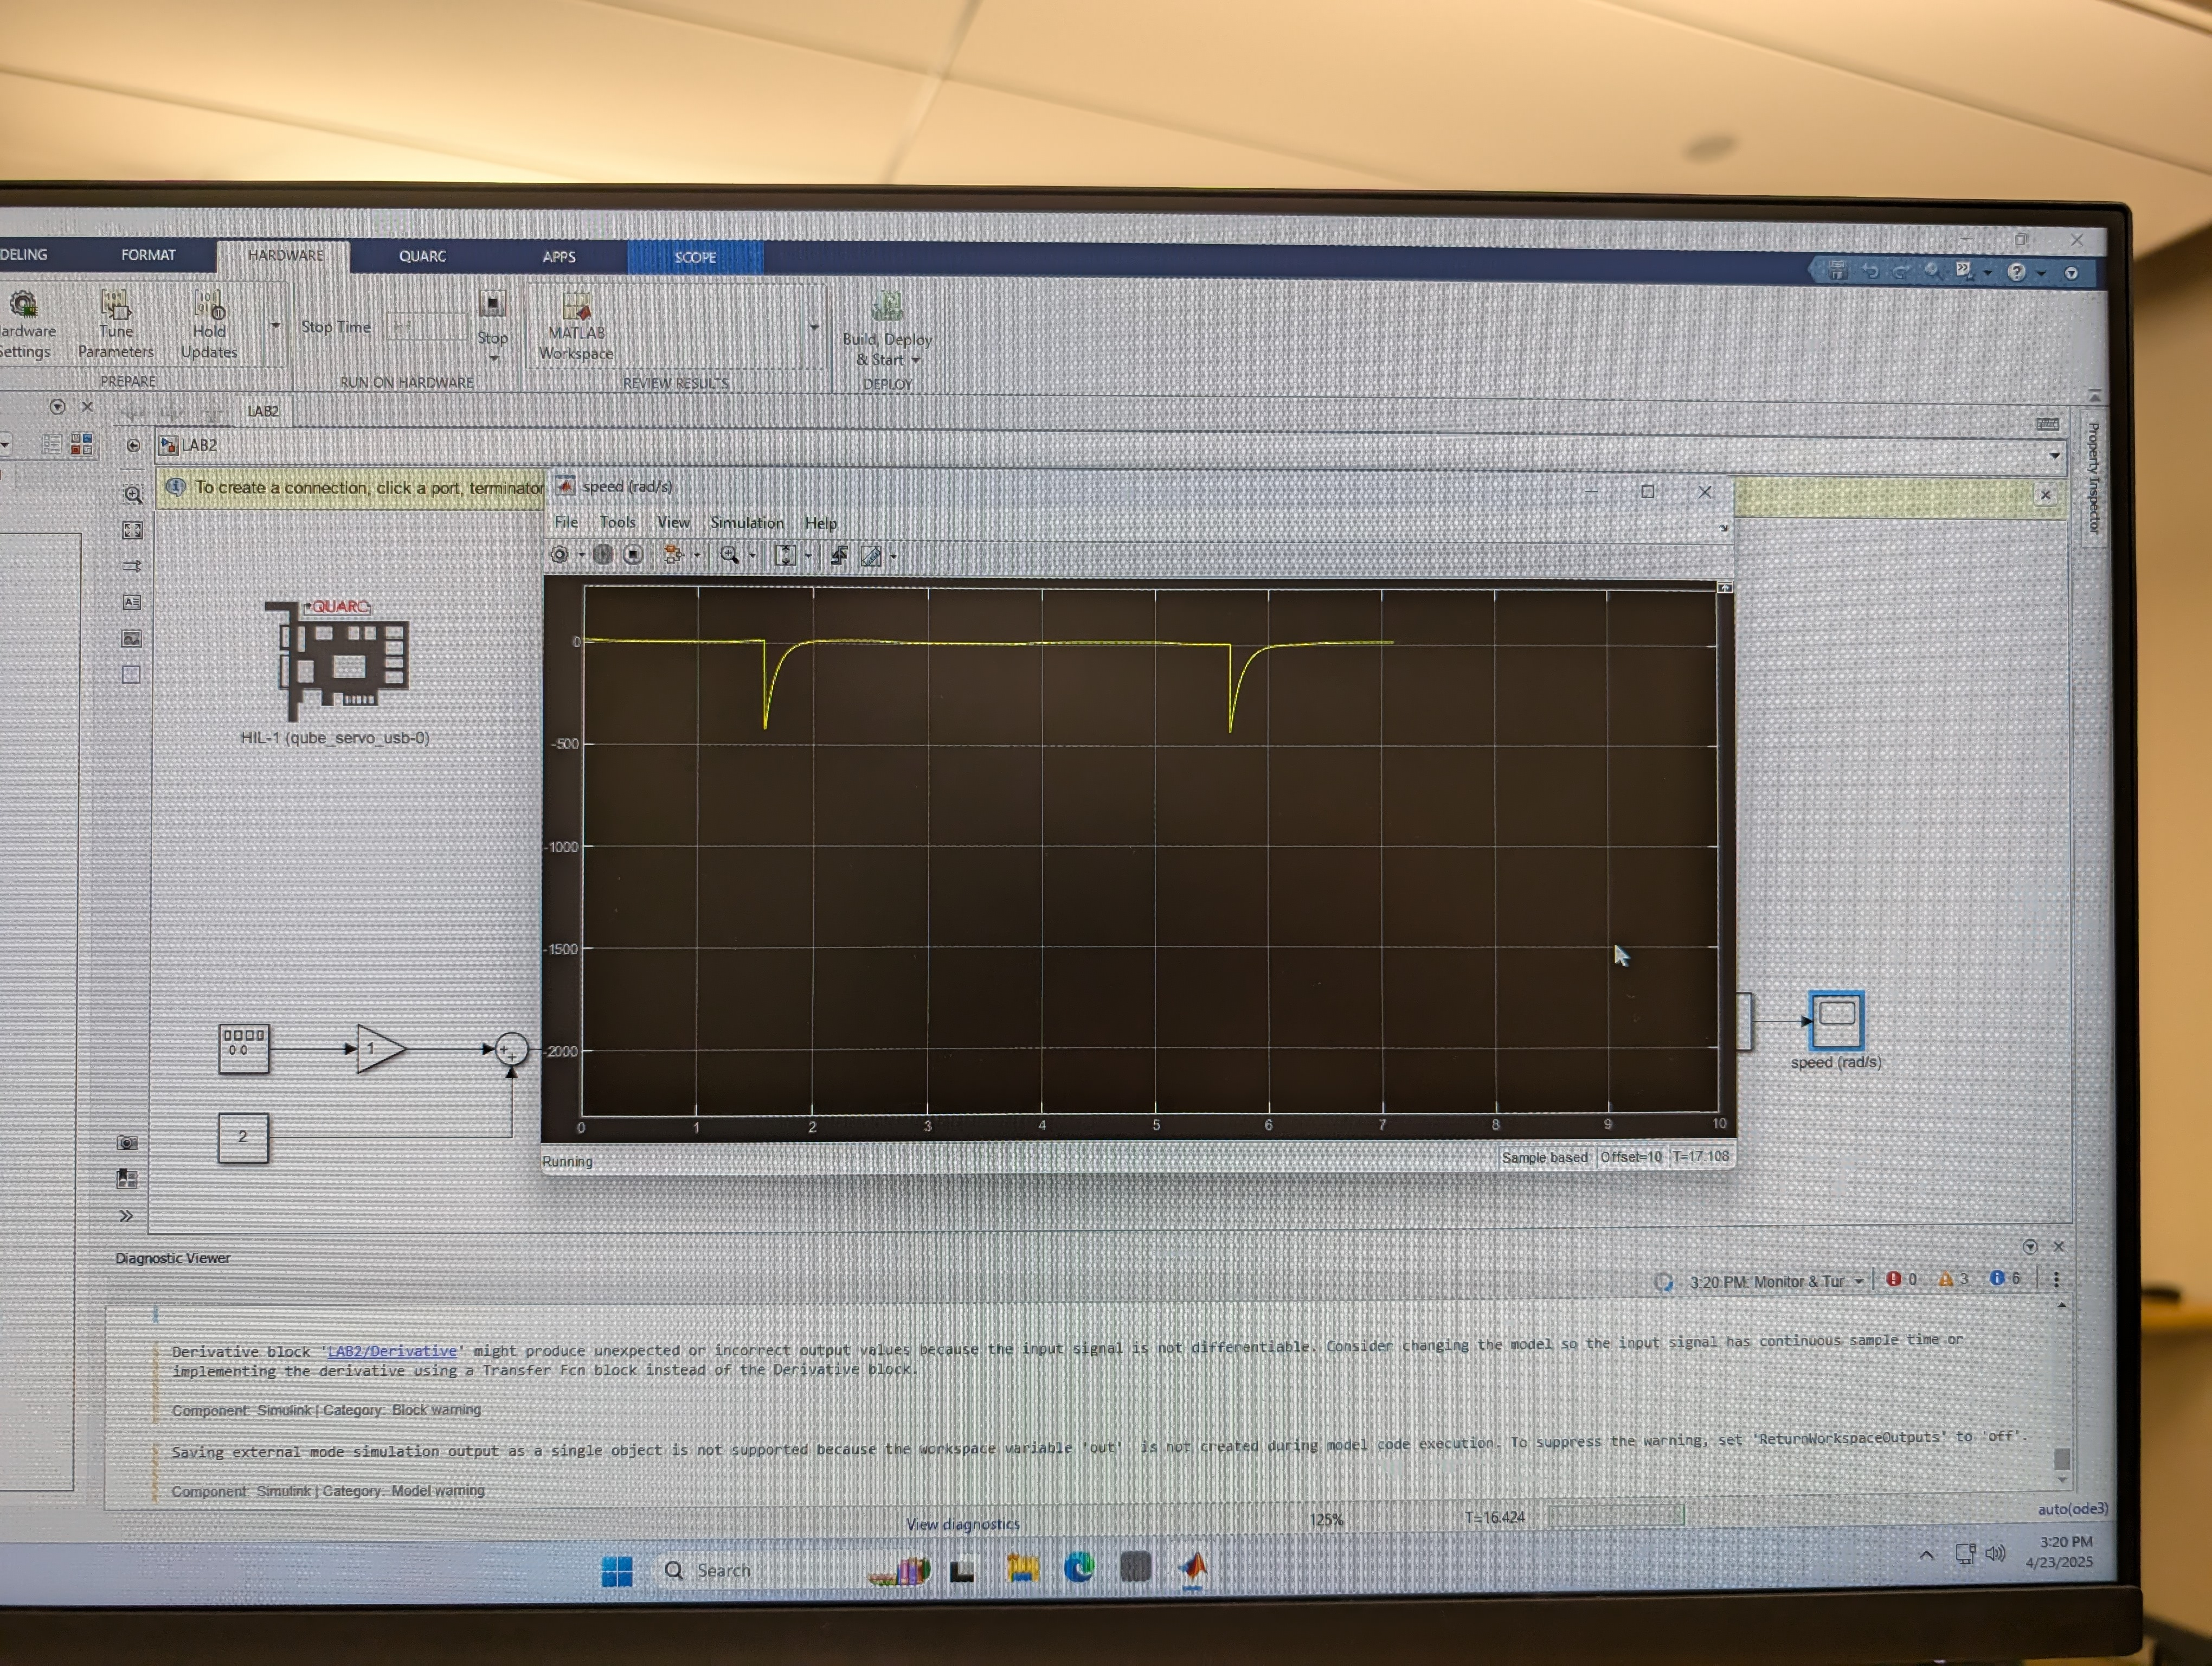
\includegraphics[width=0.49\linewidth]{6.jpg}
    \includegraphics[width=0.49\linewidth]{7.jpg}

    \centering
    \caption{Filtered response with varying $\omega_f$}
    \label{fig:4}
\end{figure}
We can see that the right plot, which uses $\omega_f=200$, is considerably more stable than both the original plot and the $\omega_f=10$ plot (on the left). When the cutoff frequency is lower, we see that the plot's response is much slower, and we still maintain massive spikes in the plot. Compared to the higher cutoff frequency, the lower frequency plot has larger spikes but is slightly quicker to respond to the changes in speed. This indicates that the tradeoff for removing a larger frequency range of noise is having slower response in our graph.

\section{Analysis}
Through our experiments, we are able to determine the importance of filtering our encoder signals and obtaining encoder-based measurements using mathematical operations. We calculated the rotational speed of our servo by taking a derivative of the angular position with respect to time. Subsequently, we discovered optimal methods for filtering our signal by analyzing the speed response in our scope and determining the frequencies to be filtered out, from which we created a transfer function to manipulate our cutoff frequency and maintain a substantially cleaner signal. One of the most critical points of knowledge that we discovered was the idea of trade-offs when using filters, specifically low-pass filters in our scenario. By manipulating $\omega_f$ in our implemented transfer function, we observed how a higher cutoff frequency can result in a cleaner signal at the cost of a much slower (thus less accurate) speed measurement.  

\section{Conclusion}
In this lab, we explored the fundamentals of calculating and filtering an encoder-based measurement, using mathematical operations and transfer functions to obtain intuitive measurements. Further, we familiarized ourselves with implementing mathematical operations such as transfer functions to our systems using Simulink and QUANSER.

\end{document}